\documentclass{beamer}
\usepackage[utf8]{inputenc}

\title{Introduction to 3D vision}
\author{Timothée Wintz}\institute{Sony CSL Paris}

\graphicspath{{images}}

\begin{document}

\begin{frame}
\titlepage
\end{frame}

\section{Camera model}

\begin{frame}
    \tableofcontents
\end{frame}

\begin{frame}
    \tableofcontents[sectionstyle=show/shaded]
\end{frame}

\begin{frame}{Pinhole camera model}
    \centering
    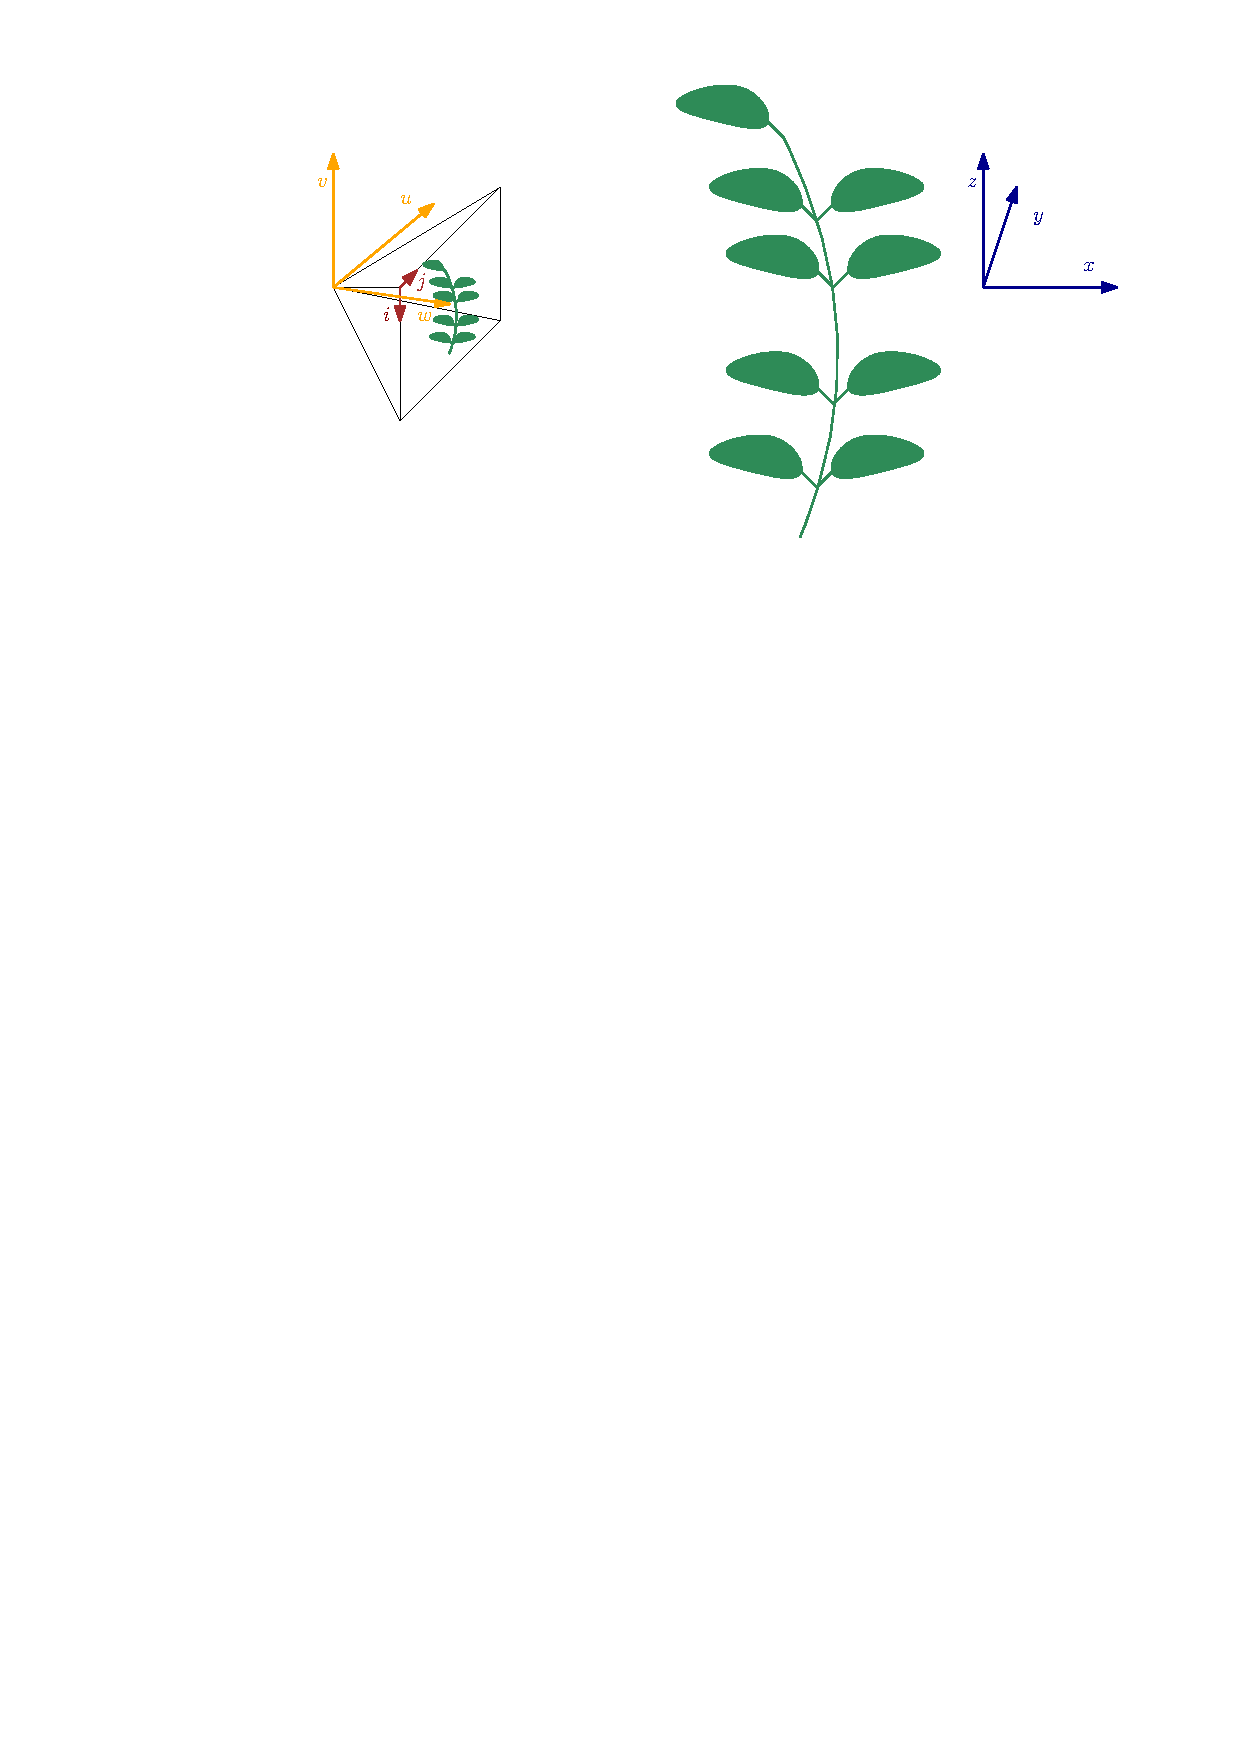
\includegraphics[width=\textwidth]{images/reperes.pdf}
\end{frame}

\begin{frame}{Camera pose}
    \centering
    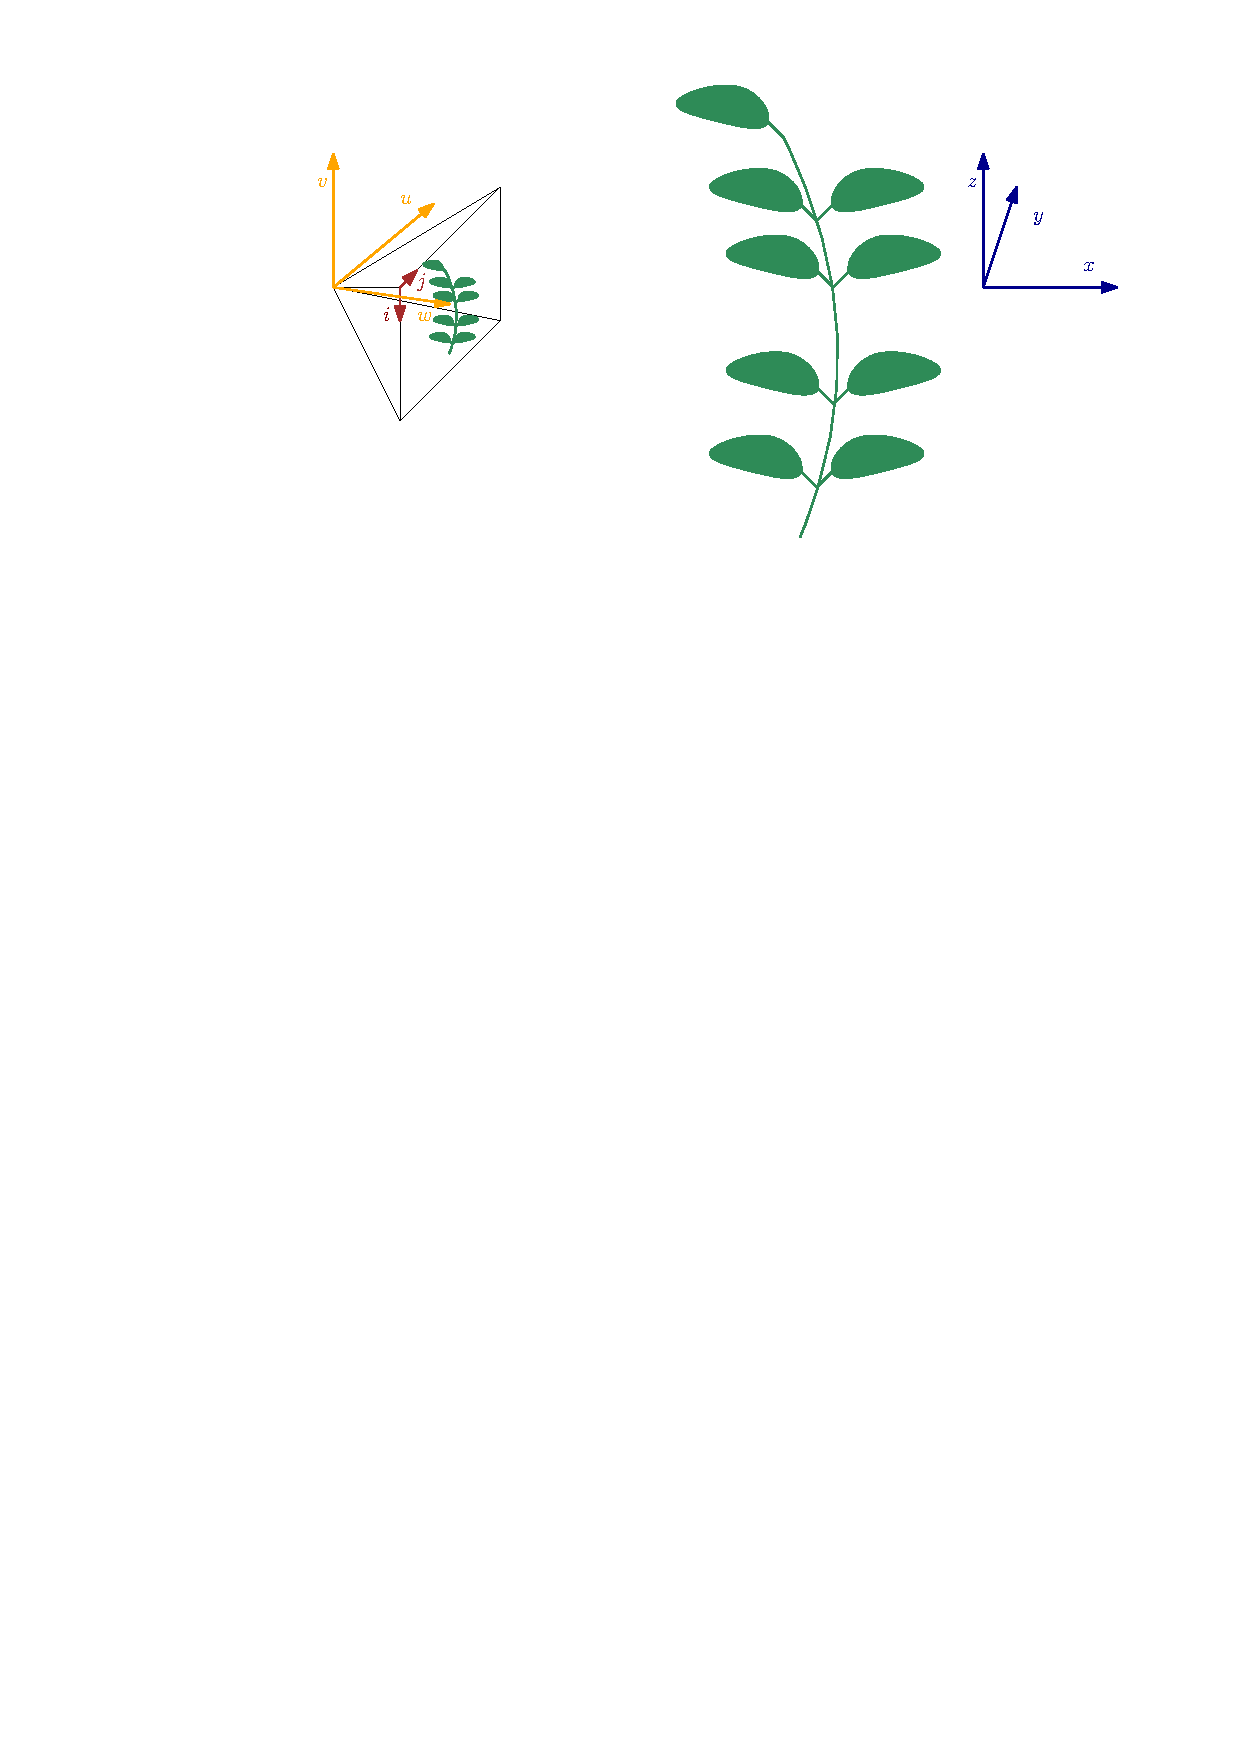
\includegraphics[width=0.7\textwidth]{images/reperes.pdf}

    Extrinsics: rotation $R$ and translation $T$.
    $$\left( \begin{array}{c}
    u \\ v \\ w
    \end{array} \right)= R\left( \begin{array}{c}
    x \\ y \\ z
    \end{array} \right) + T$$
\end{frame}

\begin{frame}{Fundamental matrix}
    \begin{columns}
        \begin{column}{0.4\textwidth}
            \centering
            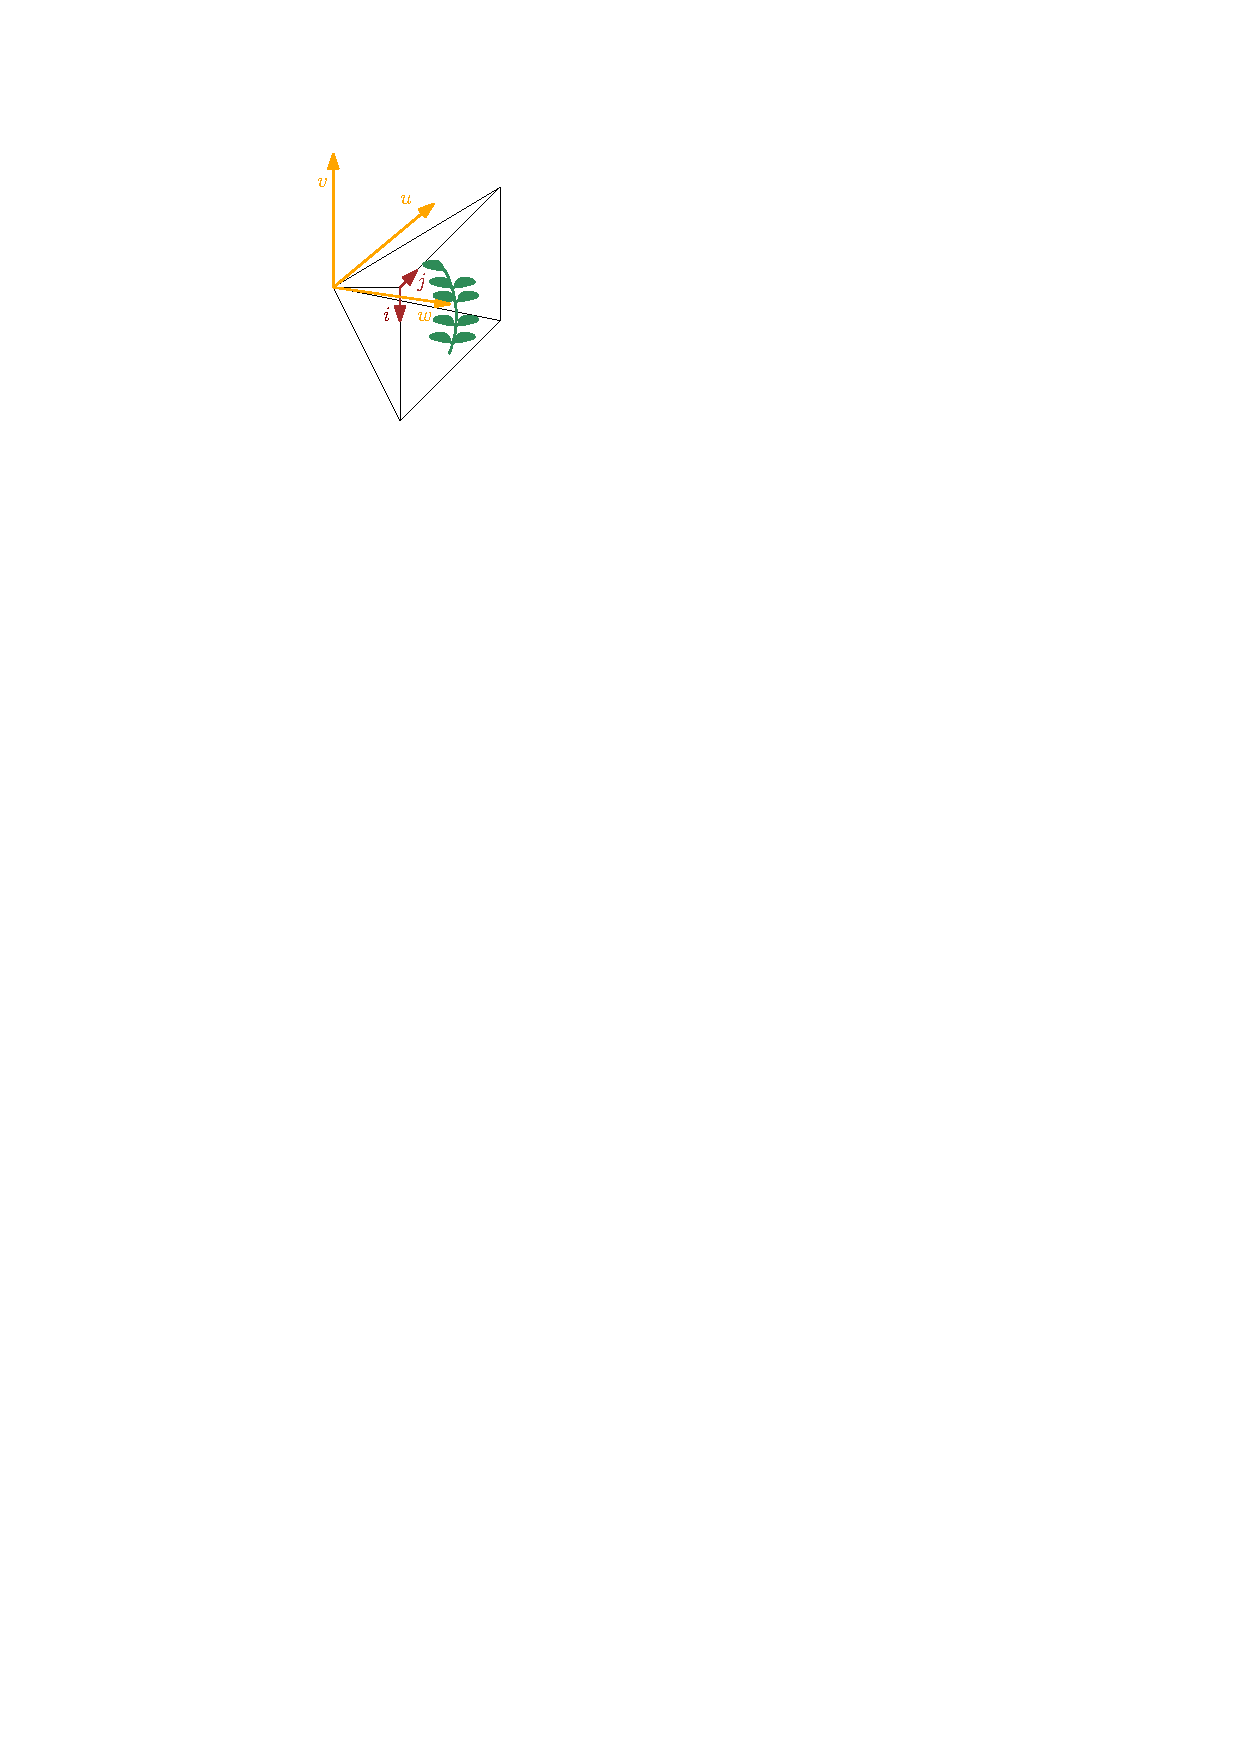
\includegraphics[width=\textwidth]{images/cam.pdf}
        \end{column}
        \begin{column}{0.6\textwidth}
            $$j = f_x \frac{u}{w} + c_x, i = f_y \frac{v}{w} + c_y$$

            $$\left( \begin{array}{c}
    j \\ i \\ 1
    \end{array} \right) = F \left( \begin{array}{c}
    u/w \\ v/w \\ 1
    \end{array} \right)$$ where

    $$F = \left( \begin{array}{ccc}
            f_x & 0 & c_x \\ 0 & f_y & c_y \\ 0 & 0 & 1
    \end{array} \right)$$
        \end{column}
    \end{columns}
\end{frame}

\begin{frame}{Pinhole camera model}
    \centering
    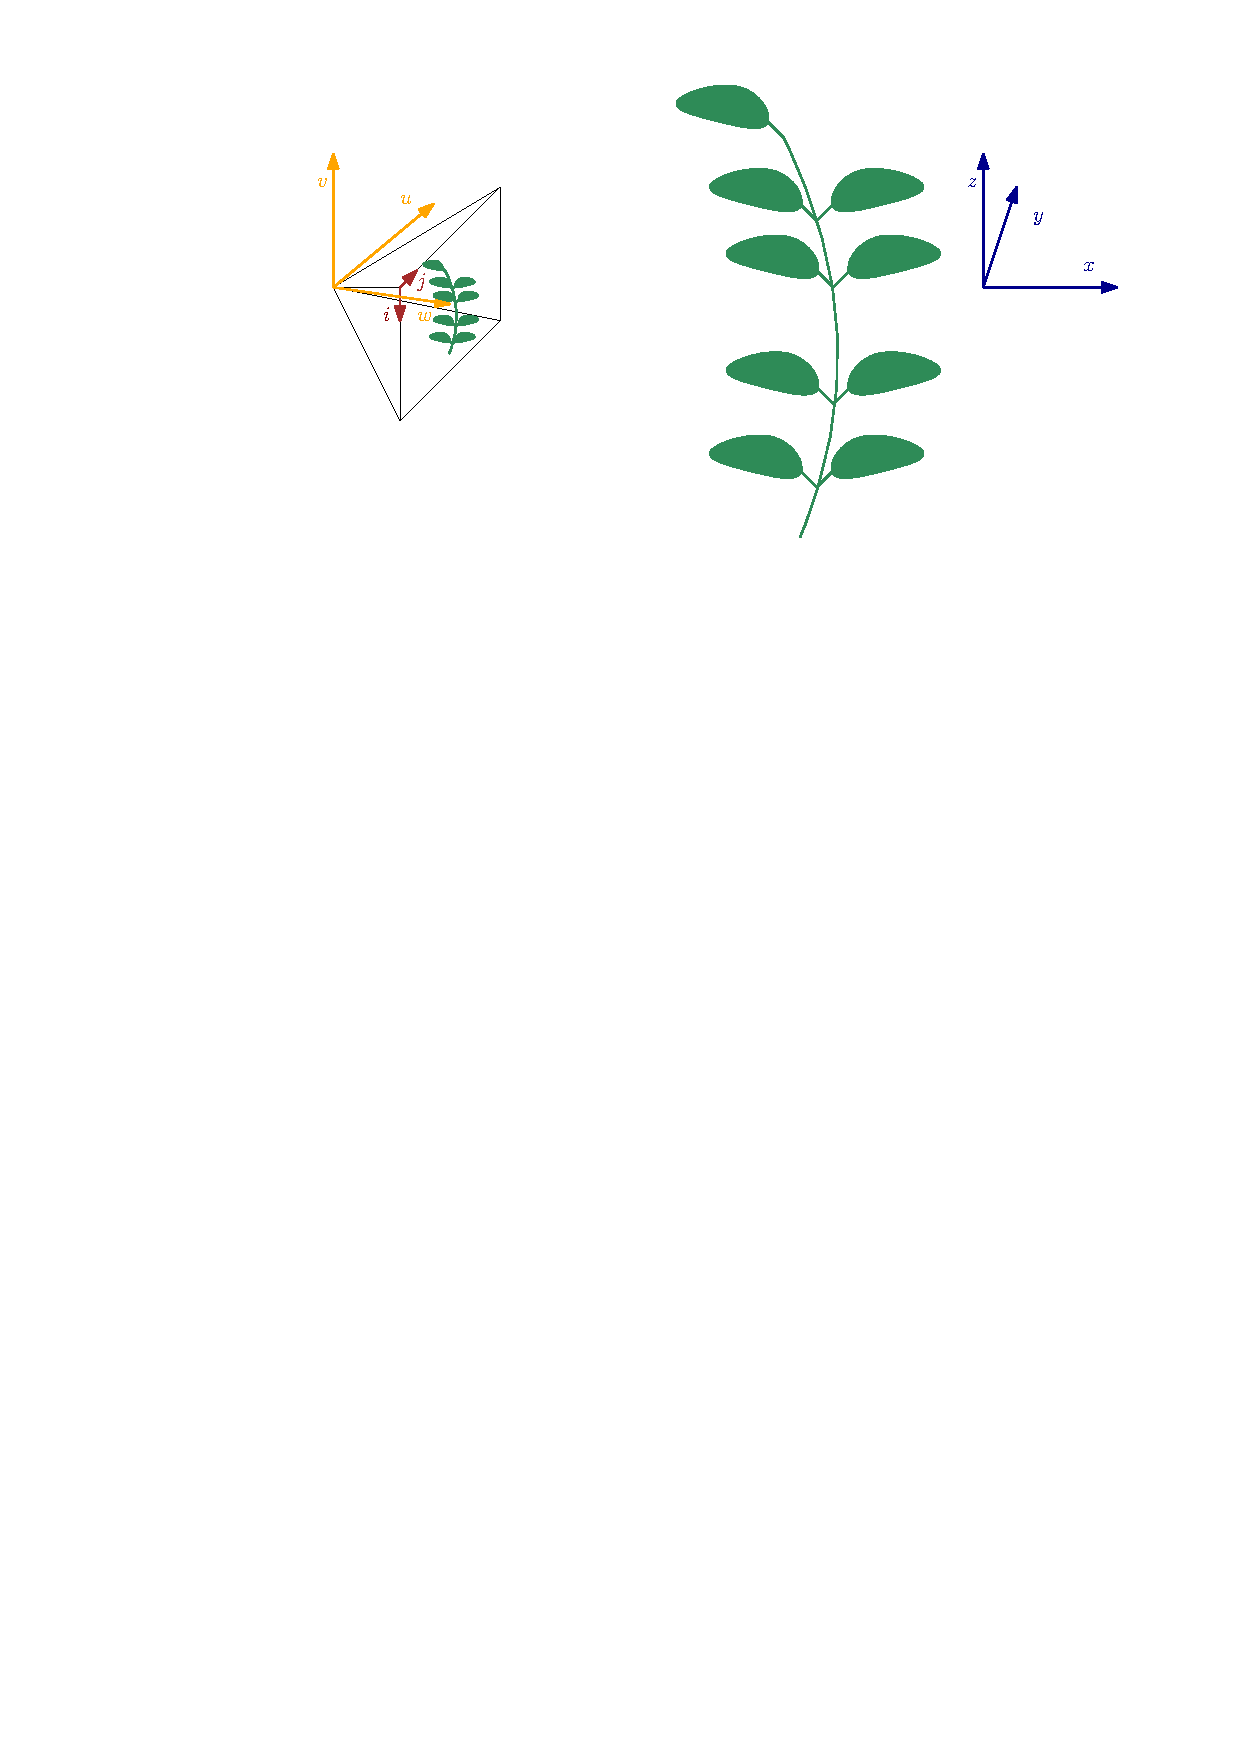
\includegraphics[width=0.6\textwidth]{images/reperes.pdf}

    Extrinsics: $\left( \begin{array}{c}
            u \\ v \\ w
            \end{array} \right)= R\left( \begin{array}{c}
            x \\ y \\ z
    \end{array} \right) + T$

    Intrinsics: $\left( \begin{array}{c}
            u \\ v \\ w
    \end{array} \right)$
\end{frame}
\begin{frame}{Camera distortion}
    \centering
    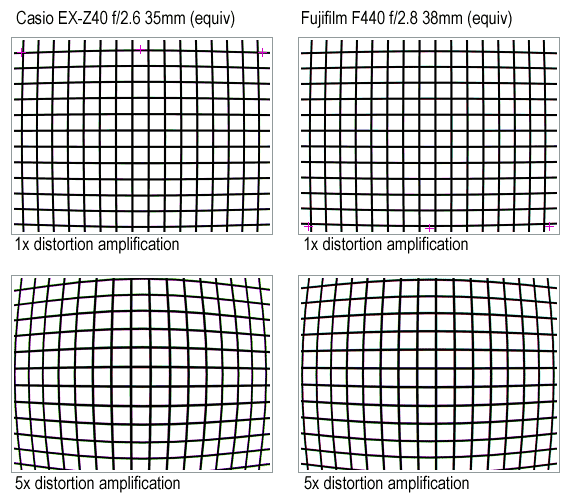
\includegraphics[width=0.3\textwidth]{images/qwe_download.png}
    \begin{block}{OpenCV model}
        \[
            r = \sqrt{x^2 + y^2}
        \]
        \[
            x_{\textrm{corrected}} = x(1+k_1r^2 + k_2r^4 + k_3r^6)
        \]
        \[
            y_{\textrm{corrected}} = x(1+k_1r^2 + k_2r^4 + k_3r^6)
        \]
        Simplified radial:
        $k_2 = k_3 = 0.$
    \end{block}

\end{frame}
\begin{frame}{Summary}
    \begin{block}{Camera parameters}
        5 to 7 parameters: $f_x, f_y, c_x, c_y, k_1, (k_2, k_3)$.
    \end{block}
    \begin{block}{Pose parameters}
        9 parameters: 6 for $R$, 3 for $T$.
    \end{block}
\end{frame}
\section{Stereo vision}
\begin{frame}
    \tableofcontents[sectionstyle=show/shaded]
\end{frame}
\begin{frame}{Basic principle}
    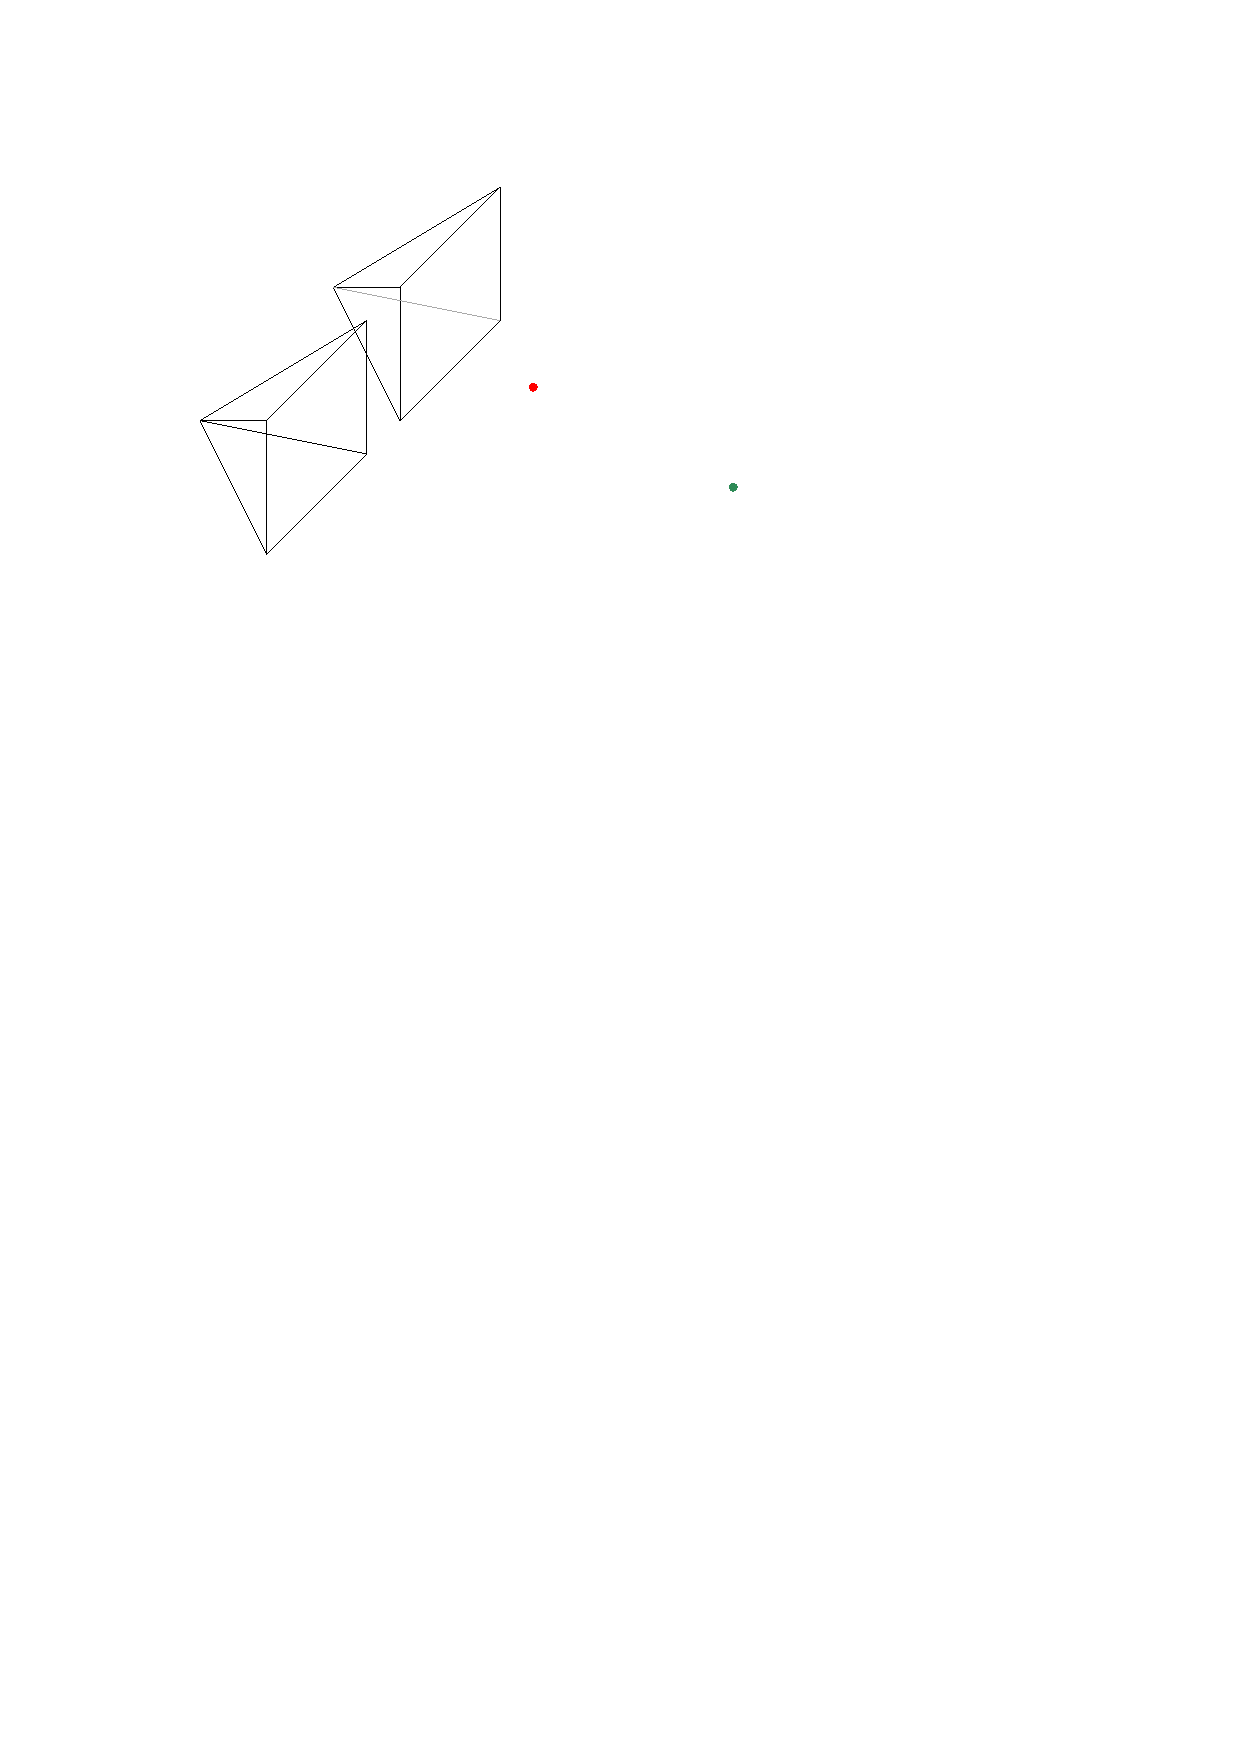
\includegraphics[width=\textwidth]{images/stereo.pdf}
\end{frame}

\begin{frame}{Basic principle}
    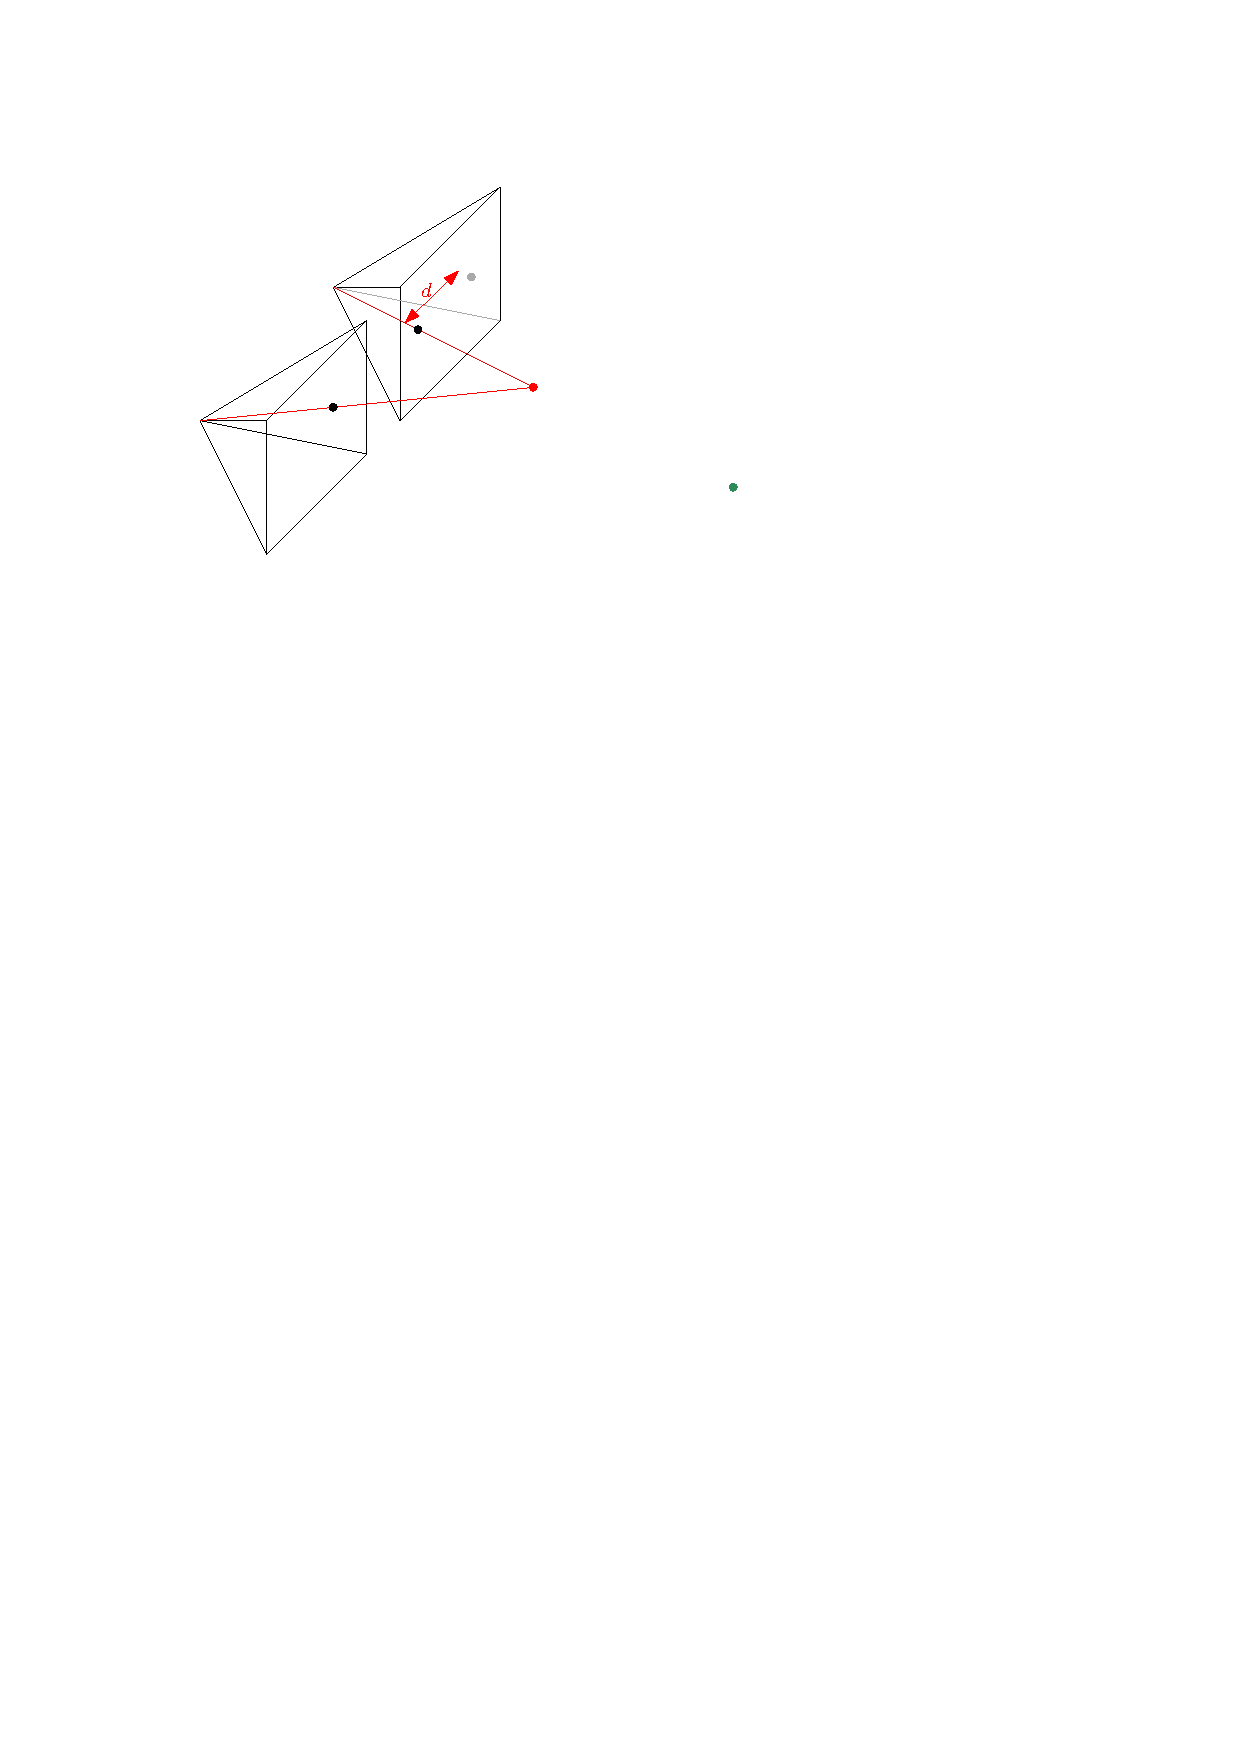
\includegraphics[width=\textwidth]{images/stereo_1.pdf}
\end{frame}

\begin{frame}{Basic principle}
    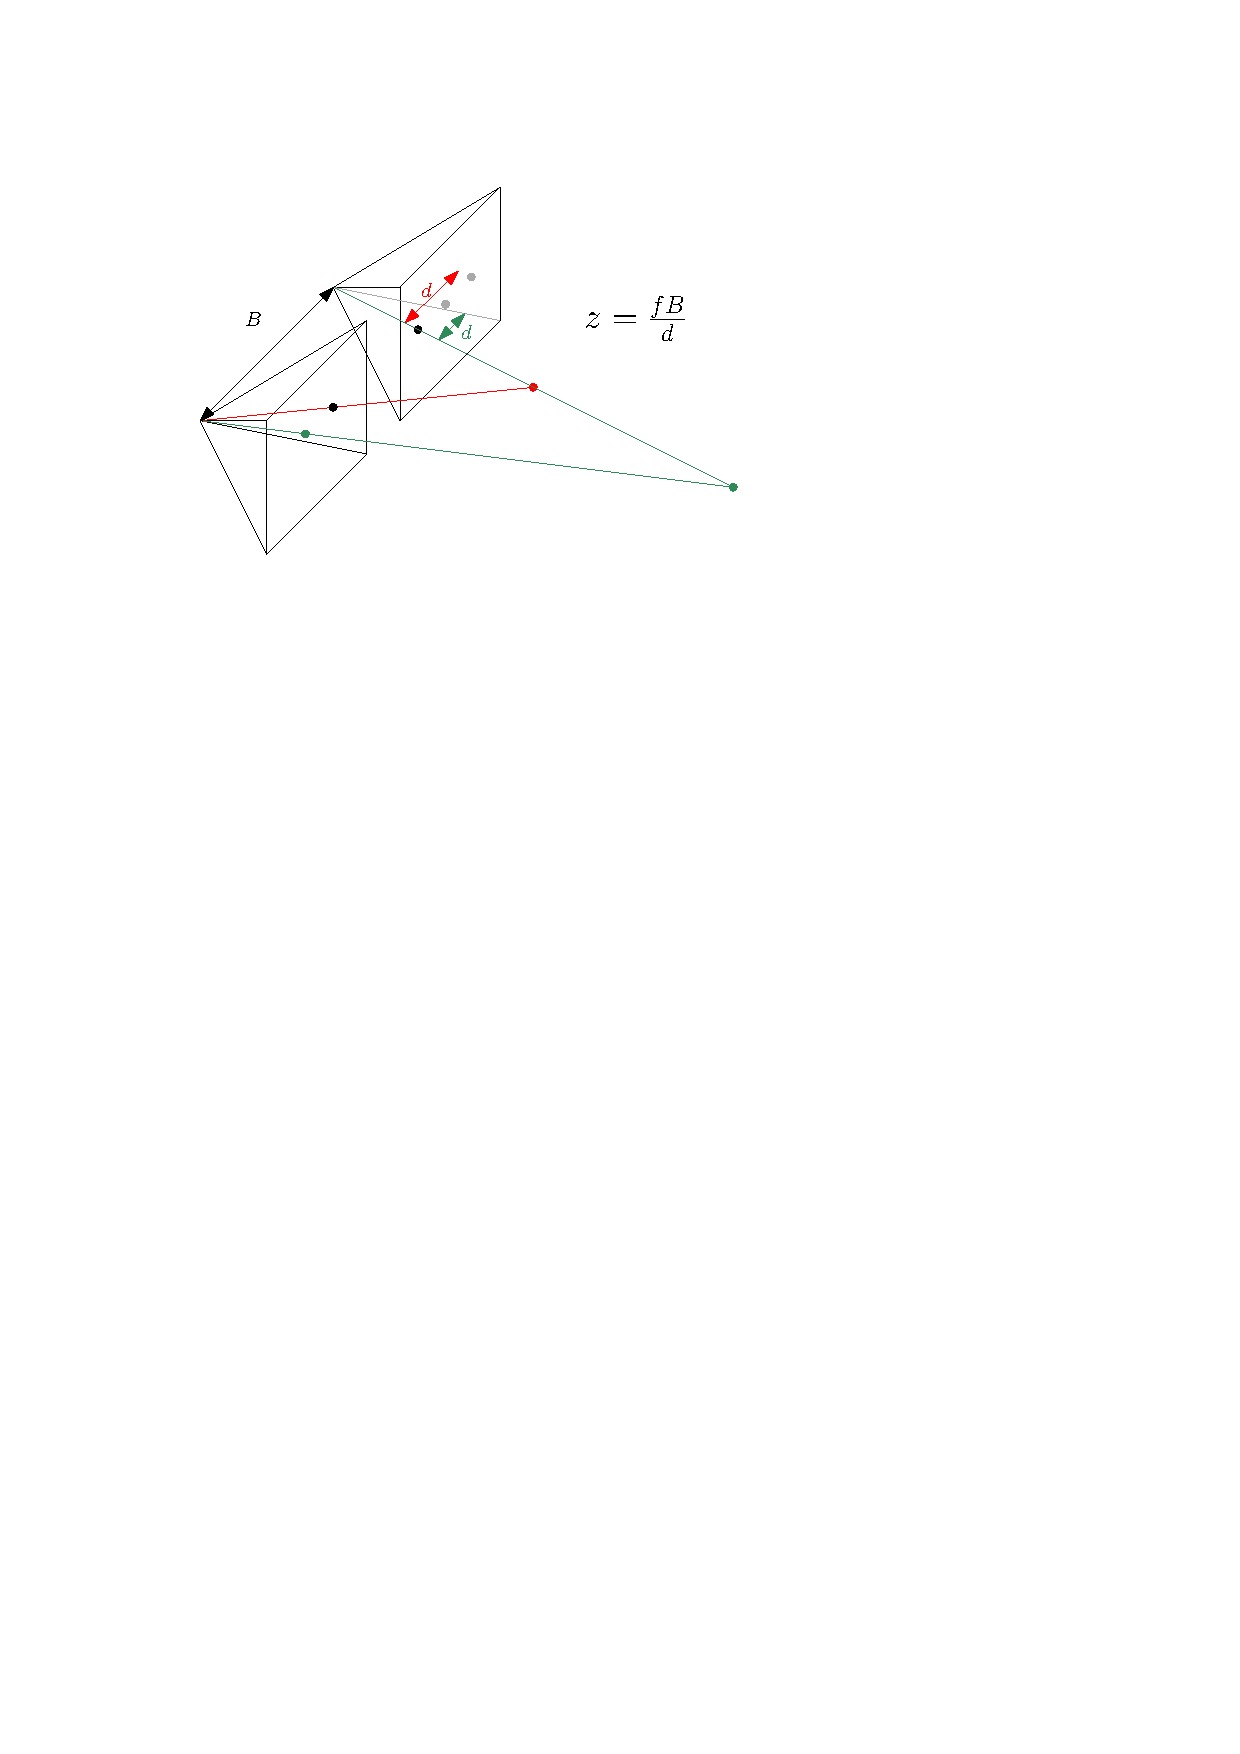
\includegraphics[width=\textwidth]{images/stereo_2.pdf}
\end{frame}


\begin{frame}{Disparity map}
    \begin{block}{Goal}
        Compute $d$ at every point in the image.
    \end{block}
    \vspace{1em}
    \centering
    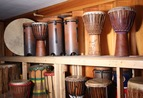
\includegraphics[width=0.3\textwidth]{images/im0.jpg}
    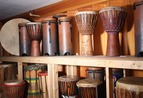
\includegraphics[width=0.3\textwidth]{images/im1.jpg}
    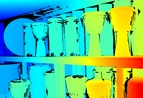
\includegraphics[width=0.3\textwidth]{images/disp0.jpg}
\end{frame}

\section{Photogrammetry}
\begin{frame}
    \tableofcontents[sectionstyle=show/shaded]
\end{frame}
\begin{frame}{Principle}
\end{frame}
\end{document}
